\clearpage

\section{공격 실행 엔진}\label{sec:operations}

\subsection{문제 정의}\label{subsec:op-problem}

실제 공격은 여러 단계의 연속적인 공격 행위로 구성될 수 있다.
정보를 수집하고, 수집한 정보를 바탕으로 다음 행동의 대상을 결정하고, 권한을 얻은 뒤 다른 호스트로 이동한다.
BAS 플랫폼에서 이러한 공격 흐름을 재현하려면 다음 세 가지 조건을 충족해야 한다.

\begin{itemize}
    \item \textbf{순서}: 이전 단계가 완료되기 전에 다음 단계 명령을 전달해서는 안 된다. 다만 에이전트는 서버의 요청 시점이 아니라 자체 비컨 주기에 맞춰 명령을 수신한다.
    \item \textbf{단계 간 데이터 전달}: 이전 단계의 출력(예: 사용자 이름, 커널 버전)을 후속 단계의 명령에 반영할 수 있어야 한다.
    \item \textbf{다중 대상 실행}: 동일한 계획을 여러 호스트에서 동시에 실행할 때, 호스트별 실행 속도와 환경(플랫폼, 셸)이 서로 다르더라도 각 호스트의 실행 상태를 독립적으로 관리할 수 있어야 한다.
\end{itemize}

\textbf{공격 실행}은 순서가 지정된 Ability 목록과 대상 에이전트 집합의 조합으로 정의되며, 각 에이전트의 진행 상태는 하나의 엔진이 관리한다.

\subsection{진행 규칙}\label{subsec:op-rules}

엔진의 핵심 규칙은 하나의 공격 실행 안에서 \textbf{에이전트별로 한 번에 최대 하나의 단계만 실행}할 수 있다는 것이다.
이 제한은 공격 실행 단위로 적용되므로, 같은 에이전트가 여러 공격 실행에 포함되어 있으면 공격 실행마다 하나씩의 단계가 동시에 진행될 수 있다.
엔진은 각 에이전트에 대해 다음 순서로 진행 여부를 판단한다.

\begin{enumerate}
    \item 해당 에이전트에 `대기' 또는 `전송됨' 상태의 단계가 있으면 해당 에이전트의 새로운 단계를 대기열에 등록하지 않는다.
    \item 그렇지 않으면 실행 계획에서 상태가 기록되지 않은 단계 중 실행 순서가 가장 앞선 단계를 선택한다.
    \item 해당 단계를 실행할 수 있으면(아래 조건) 명령을 생성하여 대기열에 등록한 후 해당 에이전트에 대한 진행 판단을 종료한다.
    \item 실행할 수 없으면 상태를 `건너뜀'으로 기록하고, 다음 단계에 대해 3번 절차를 반복한다.
\end{enumerate}

모든 대상 에이전트의 실행 단계가 `완료', `시간 초과', `건너뜀' 중 하나로 기록되면 공격 실행 상태를 `종료'로 변경한다.
`시간 초과' 상태는 정의되어 있으나, 현재는 시간 초과 여부를 자동으로 판정하는 기능을 지원하지 않는다.
따라서 명령 전송 이후 실행 결과가 수신되지 않으면 해당 단계가 `전송됨' 상태에 머물러 후속 단계가 진행되지 않을 수 있다.

한 단계를 실행할 수 없는 경우는 다음과 같다.

\begin{itemize}
    \item 실행 계획에 포함된 Ability가 라이브러리에서 삭제된 경우.
    \item 해당 Ability에 정의된 실행기 중 에이전트가 지원하는 실행기가 없는 경우(\ref{subsec:ability}절).
    \item 명령 실행에 필요한 변수의 값이 지정되지 않은 경우(\ref{subsec:facts}절).
    \item 해당 에이전트가 운영 콘솔에서 삭제된 경우. 이때는 그 에이전트의 남은 단계의 상태를 모두 `건너뜀'으로 기록하여, 삭제된 에이전트로 인해 공격 실행이 종료되지 않는 상황을 방지한다.
\end{itemize}

그림~\ref{fig:step-states}은 에이전트별 실행 단계의 상태 전이 과정을 나타낸다.

\begin{figure}[H]
\centering
\begin{tikzpicture}[every node/.style={font=\footnotesize}]
  \node[ext, minimum width=18mm] (none) at (0,0) {기록 없음};
  \node[box, minimum width=18mm] (q) at (3.6,0) {대기};
  \node[box, minimum width=18mm] (s) at (8.3,0) {전송됨};
  \node[box, minimum width=18mm] (c) at (12.3,0) {완료};
  \node[ext, minimum width=18mm] (k) at (3.6,-2.0) {건너뜀};
  \node[ext, minimum width=18mm, dashed] (t) at (12.3,-2.0) {시간 초과};
  \draw[arr] (none) -- node[lbl, above]{실행 가능} (q);
  \draw[arr] (q) -- node[lbl, above]{정기 비컨에서 전달} (s);
  \draw[arr] (s) -- node[lbl, above]{결과 도착} (c);
  \draw[arr] (none) |- node[lbl, below, pos=0.75]{실행 불가} (k);
  \draw[arr, dashed] (s) -- (t);
  \node[lbl, anchor=north] at (t.south) {(현재 미사용)};
  \node[lbl] at (6.15,-3.2) {종료 상태: 완료 · 건너뜀 · 시간 초과 \quad $\Rightarrow$ \quad 후속 단계 실행 여부 판단};
\end{tikzpicture}
\caption{에이전트별 실행 단계의 상태 전이}
\label{fig:step-states}
\end{figure}

\paragraph{\textbf{엔진 호출 시점:}}
엔진은 별도의 주기 작업 없이 다음 두 가지 이벤트가 발생할 때 호출된다.
하나는 운영자가 공격 실행을 시작하거나 재개할 때(콘솔)이고, 다른 하나는 공격 실행 단계의 결과가 도착했을 때(C2)이다.
C2는 결과를 저장한 직후 엔진을 실행해 다음 단계를 대기열에 등록한다.
다만 해당 단계의 명령은 결과 보고에 대한 응답에 포함하지 않는다. 에이전트는 결과 보고에 대한 응답을 처리하지 않으므로, 해당 응답에 명령을 포함하면 상태만 `전송됨'으로 변경되고 명령은 실제로 수신되지 않기 때문이다.
다음 단계는 에이전트의 다음 정기 비컨에서 전달되므로, 단계 간 대기 시간은 일반적으로 비컨 간격에 해당한다(터미널이 열려 있으면 약 1초).

엔진은 데이터베이스에 기록된 현재 실행 상태를 기준으로 판단하며, 진행 중인 단계가 있는 에이전트에는 새 단계를 등록하지 않는다.
따라서 운영 콘솔과 C2 서버는 동일한 진행 규칙을 사용하며, 같은 실행 상태에서 엔진을 순차적으로 반복 호출하더라도 단계가 중복 등록되지 않는다.

\paragraph{\textbf{에이전트 간 독립 진행:}}
각 에이전트는 다른 에이전트의 진행 상태와 관계없이 독립적으로 실행된다.
에이전트별 처리 속도와 비컨 간격에 따라 동일한 실행 계획의 완료 시점은 달라질 수 있다.
결과 화면은 에이전트를 행, 실행 단계를 열로 배치한 격자로 진행 상태를 표시한다(\ref{subsec:op-screens}절).

\paragraph{\textbf{오류 시 중단:}}
`건너뜀/실패 시 해당 에이전트의 남은 단계 중단' 옵션을 활성화한 경우, 특정 에이전트의 실행 단계가 `건너뜀'으로 처리되면 해당 에이전트의 남은 단계도 모두 `건너뜀'으로 기록한다.
이는 선행 단계의 실행 결과에 의존하는 계획(예: 수집된 정보를 후속 단계에서 활용하는 경우)에서 필요한 선행 조건을 충족하지 못한 후속 단계의 실행을 방지하기 위한 것이다.
중단 여부는 `건너뜀' 상태를 기준으로 판단한다. 명령이 0이 아닌 종료 코드를 반환한 단계는 `완료'로 기록되며, 종료 코드와 출력은 결과 화면에서 확인할 수 있다.

\paragraph{\textbf{일시 중지·재개·중지:}}
`일시 중지'하면 엔진은 새로운 단계를 대기열에 등록하지 않는다. `재개' 시 엔진을 호출하여 중단된 시점의 실행 상태를 기준으로 후속 단계를 진행한다.
`중지' 시 공격 실행 상태를 `종료'로 변경한다.
다만 이미 대기열에 등록된 단계는 취소되지 않으므로, 일시 중지하거나 중지한 이후에도 다음 비컨에서 해당 단계가 실행될 수 있다.

\subsection{변수 저장소}\label{subsec:facts}

Ability 명령문에는 \texttt{\#\{host.user.name\}}과 같은 변수 치환을 위한 참조 표현을 사용할 수 있다.
공격 실행별로 하나의 \textbf{변수 저장소}를 구성하며, 변수 값은 다음 세 가지 방식으로 설정된다(그림~\ref{fig:facts}).

\begin{itemize}
    \item \textbf{운영자 입력}: 공격 실행 구성 시 `필요한 변수' 항목에 운영자가 직접 입력한 값.
    \item \textbf{에이전트 고유 값}: 에이전트 식별자, 호스트 이름, 플랫폼, 그룹, 실행 위치, C2 주소처럼 에이전트가 비컨을 통해 보고한 정보. 별도 입력이 필요하지 않으므로 운영자 입력 항목에서 제외된다.
    \item \textbf{출력에서 추출}: 각 단계에서 `+ 출력에서 변수 추출' 기능을 이용해 변수 이름과 정규표현식을 설정할 수 있다. 단계의 출력이 도착하면 정규표현식의 첫 번째 캡처 그룹을 해당 변수의 값으로 저장하며, 캡처 그룹이 없으면 일치하는 전체 문자열을 저장한다.
\end{itemize}

\begin{figure}[H]
\centering
\begin{tikzpicture}[every node/.style={font=\footnotesize}]
  \node[ext, minimum width=24mm] (u) at (0,0) {운영자 입력};
  \node[box, minimum width=24mm, minimum height=12mm] (fs) at (4.3,0) {변수 저장소\\\scriptsize 공격 실행 단위};
  \node[box, minimum width=24mm, minimum height=12mm] (sub) at (8.6,0) {명령 생성\\\scriptsize 변수 값 치환};
  \node[hot, minimum width=24mm, minimum height=12mm] (run) at (12.9,0) {에이전트 실행};
  \node[ext, minimum width=28mm] (a) at (8.6,2.0) {에이전트 고유 값\\\scriptsize 호스트 · 플랫폼 · C2 주소 등};
  \node[box, minimum width=24mm] (cap) at (8.6,-2.1) {추출 규칙\\\scriptsize 정규식 · 첫 캡처 그룹};

  \draw[arr] (u) -- (fs);
  \draw[arr] (fs) -- node[lbl, above]{저장된 값} (sub);
  \draw[arr] (a) -- node[lbl, right]{단계별 참조} (sub);
  \draw[arr] (sub) -- node[lbl, above]{명령} (run);
  \draw[arr] (run) |- node[lbl, right, pos=0.25]{출력} (cap);
  \draw[arr] (cap) -| node[lbl, below, pos=0.25]{추출된 값} (fs);
\end{tikzpicture}
\caption{변수 저장소를 통한 단계 간 값 전달}
\label{fig:facts}
\end{figure}

명령을 생성할 때 값이 지정되지 않은 변수가 하나라도 남아 있으면 해당 단계를 `건너뜀'으로 기록한다.
이는 불완전한 명령의 실행을 방지하고, 실행되지 않은 원인을 명확히 기록하기 위한 것이다.
필요한 변수를 입력하지 않으면 앞 단계의 출력에서 해당 값이 추출될 것으로 간주하며, 실행 시점까지 값이 설정되지 않으면 해당 단계는 `건너뜀'으로 기록된다.

변수 저장소는 개별 공격 실행 단위로 관리되며, 해당 공격 실행에 포함된 모든 에이전트가 공유한다.
여러 에이전트가 동일한 이름의 변수를 추출하면 나중에 수신된 값이 기존 값을 덮어쓴다.
에이전트별로 서로 다른 값을 후속 단계에 전달해야 하는 경우에는 에이전트별로 공격 실행을 나누어 구성한다.

\paragraph{\textbf{페이로드 확인:}}
공격 실행을 구성할 때 콘솔은 실행 계획에 포함된 각 Ability가 참조하는 페이로드 파일이 C2 서버에 저장되어 있는지 확인한다.
이를 위해 콘솔은 C2 서버에서 페이로드 파일 목록을 조회하며, 이는 콘솔이 C2 서버에 직접 요청하는 유일한 경우이다.
누락된 페이로드 파일이 있으면 경고 메시지를 표시한다. 필요한 페이로드가 없으면 대상 호스트에서 해당 단계의 실행이 실패할 수 있기 때문이다.
C2 서버에 접속할 수 없으면 페이로드 존재 여부를 확인할 수 없다는 안내 메시지를 표시한다.

\subsection{공격 실행 구성 및 결과 확인}\label{subsec:op-screens}

`공격 실행' 화면에서 `새 공격 실행' 버튼을 클릭하면 그림~\ref{fig:builder}의 구성 창이 열린다.
왼쪽에서 이름과 `대상 에이전트'를 지정하고 `Ability 추가'에서 절차를 검색·선택하면 오른쪽 `실행 계획'에 선택한 순서대로 표시된다.
그림의 예에서는 첫 단계(커널 정보 조회)에 커널 버전을 추출하는 규칙을 추가했으며, 마지막 단계(파일 찾기)의 실행에 필요한 변수 \texttt{host.print.file}에는 운영자가 값을 입력하였다.

\begin{figure}[H]
\centering
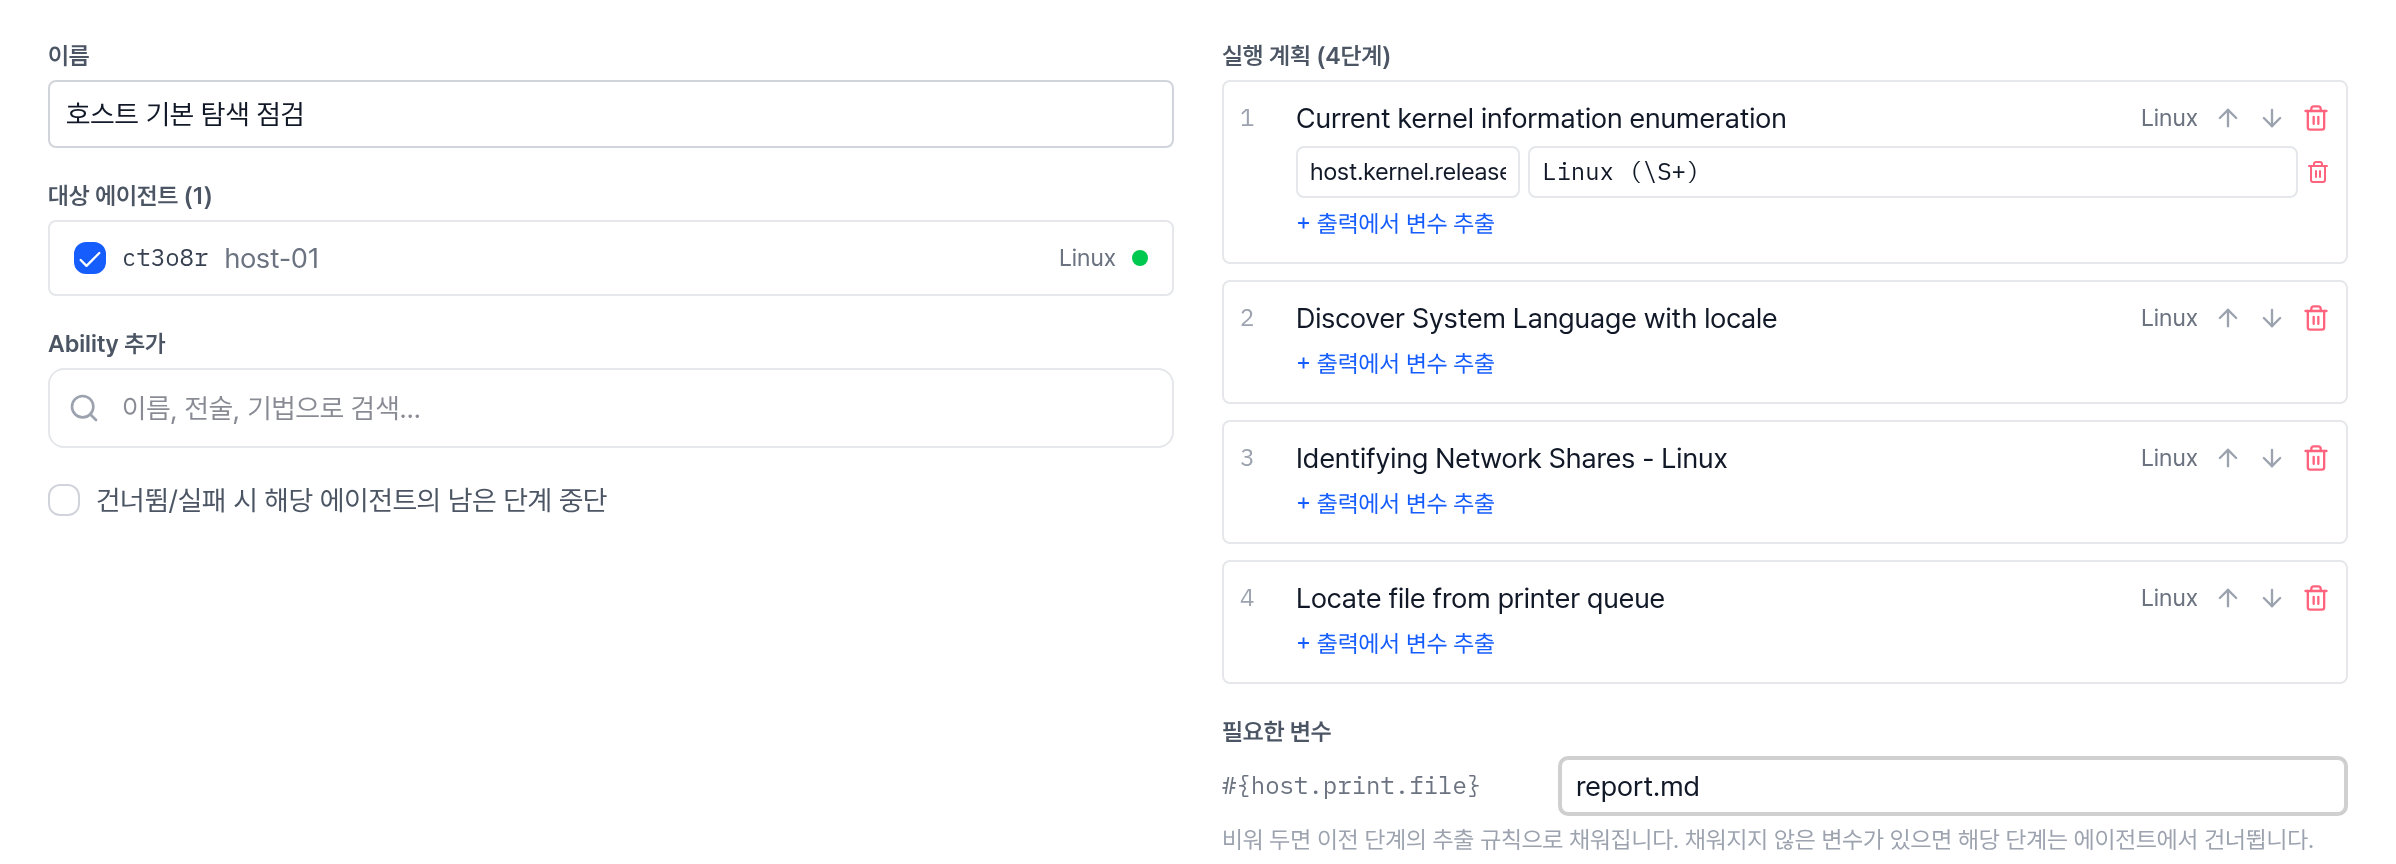
\includegraphics[width=0.7\textwidth]{screenshots-bas/builder.png}
\caption{새 공격 실행 구성 창(추출 규칙과 필요한 변수 입력)}
\label{fig:builder}
\end{figure}

`시작' 버튼을 클릭하면 공격 실행이 생성되고, 각 대상 에이전트에서 실행 가능한 첫 번째 단계가 즉시 대기열에 등록된다. 앞선 단계를 실행할 수 없으면 해당 단계는 `건너뜀'으로 기록된다. 다만 `건너뜀/실패 시 해당 에이전트의 남은 단계 중단' 옵션이 활성화된 경우에는 \ref{subsec:op-rules}절의 중단 규칙을 적용한다.
상세 화면(그림~\ref{fig:op-detail})은 에이전트를 행, 실행 단계를 열로 구성한 격자로 에이전트별 실행 단계의 상태를 표시하며, 개별 단계를 선택하면 해당 단계의 실행기, 종료 코드 및 실행 결과가 화면 하단에 표시된다.
격자 아래의 변수 저장소에는 운영자가 입력한 값과 출력에서 추출된 값이 함께 나타난다.
그림에서 \texttt{host.kernel.release}는 첫 단계의 출력 ``Linux 6.8.0-90-generic x86\_64''에 추출 규칙을 적용하여 얻은 값이다.

\begin{figure}[H]
\centering
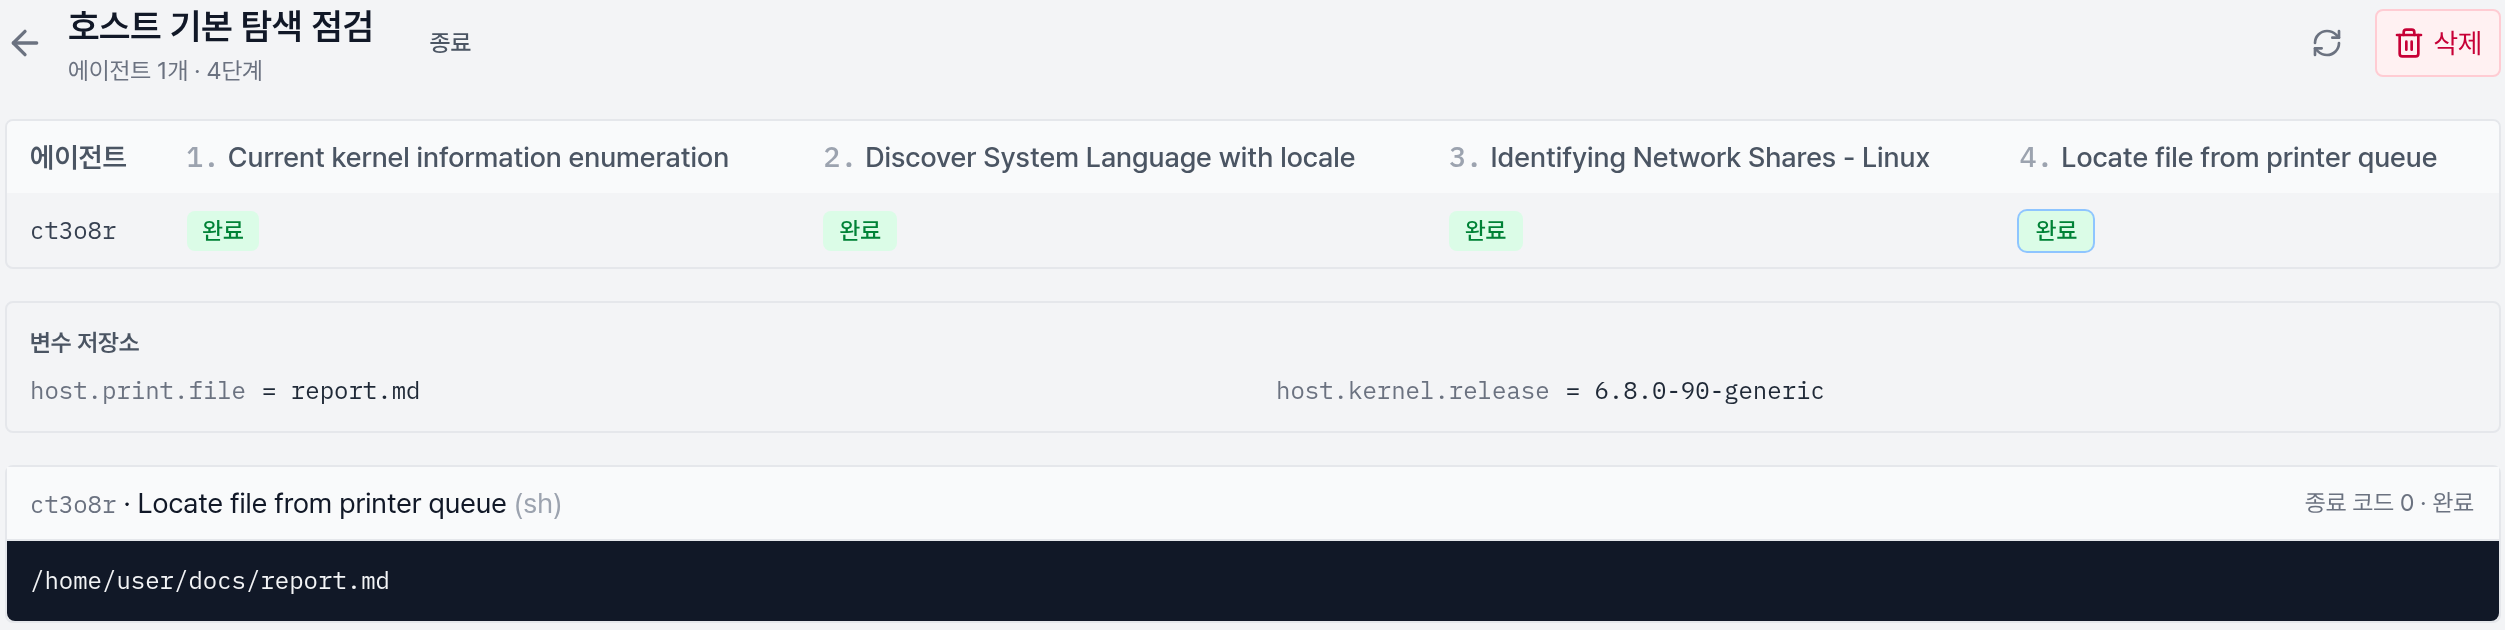
\includegraphics[width=0.9\textwidth]{screenshots-bas/ops_detail_c.png}
\caption{공격 실행 상세 화면(시험 호스트 에이전트 1개, 4단계)}
\label{fig:op-detail}
\end{figure}

그림~\ref{fig:op-detail}의 공격 실행 결과에서는 네 단계 모두 `완료' 상태로 기록되었다.
마지막 단계에서는 운영자가 입력한 변수 값을 명령문에 반영하여 해당 파일의 경로를 조회하였다.
다만 `완료'는 명령 실행 결과가 수신되었음을 의미할 뿐, 공격 성공을 의미하지는 않는다. 종료 코드가 0이 아닌 경우에도 해당 단계는 `완료'로 기록되므로, 실제 명령의 성공 여부는 종료 코드와 실행 결과를 종합적으로 검토하여 판단해야 한다.

\clearpage
\subsection{평가 계획}\label{subsec:assessment}

\textbf{평가}는 반복 수행할 시험 계획을 등록하고 관리하는 기능이다.
평가 등록 시 이름, 평가 대상(설명용 문구), 반복 횟수, 실행할 Ability와 실행 순서, 대상 에이전트를 지정한다.
현재 반복 횟수는 평가 계획의 설정값으로 관리되며, 자동 반복 실행에는 적용되지 않는다.
평가 상세 화면에서는 등록된 Ability와 해당 전술·기법을 확인할 수 있으며(그림~\ref{fig:assessment}), 평가 등록 이후 라이브러리에서 삭제된 Ability는 별도로 표시된다.


\begin{figure}[H]
\centering
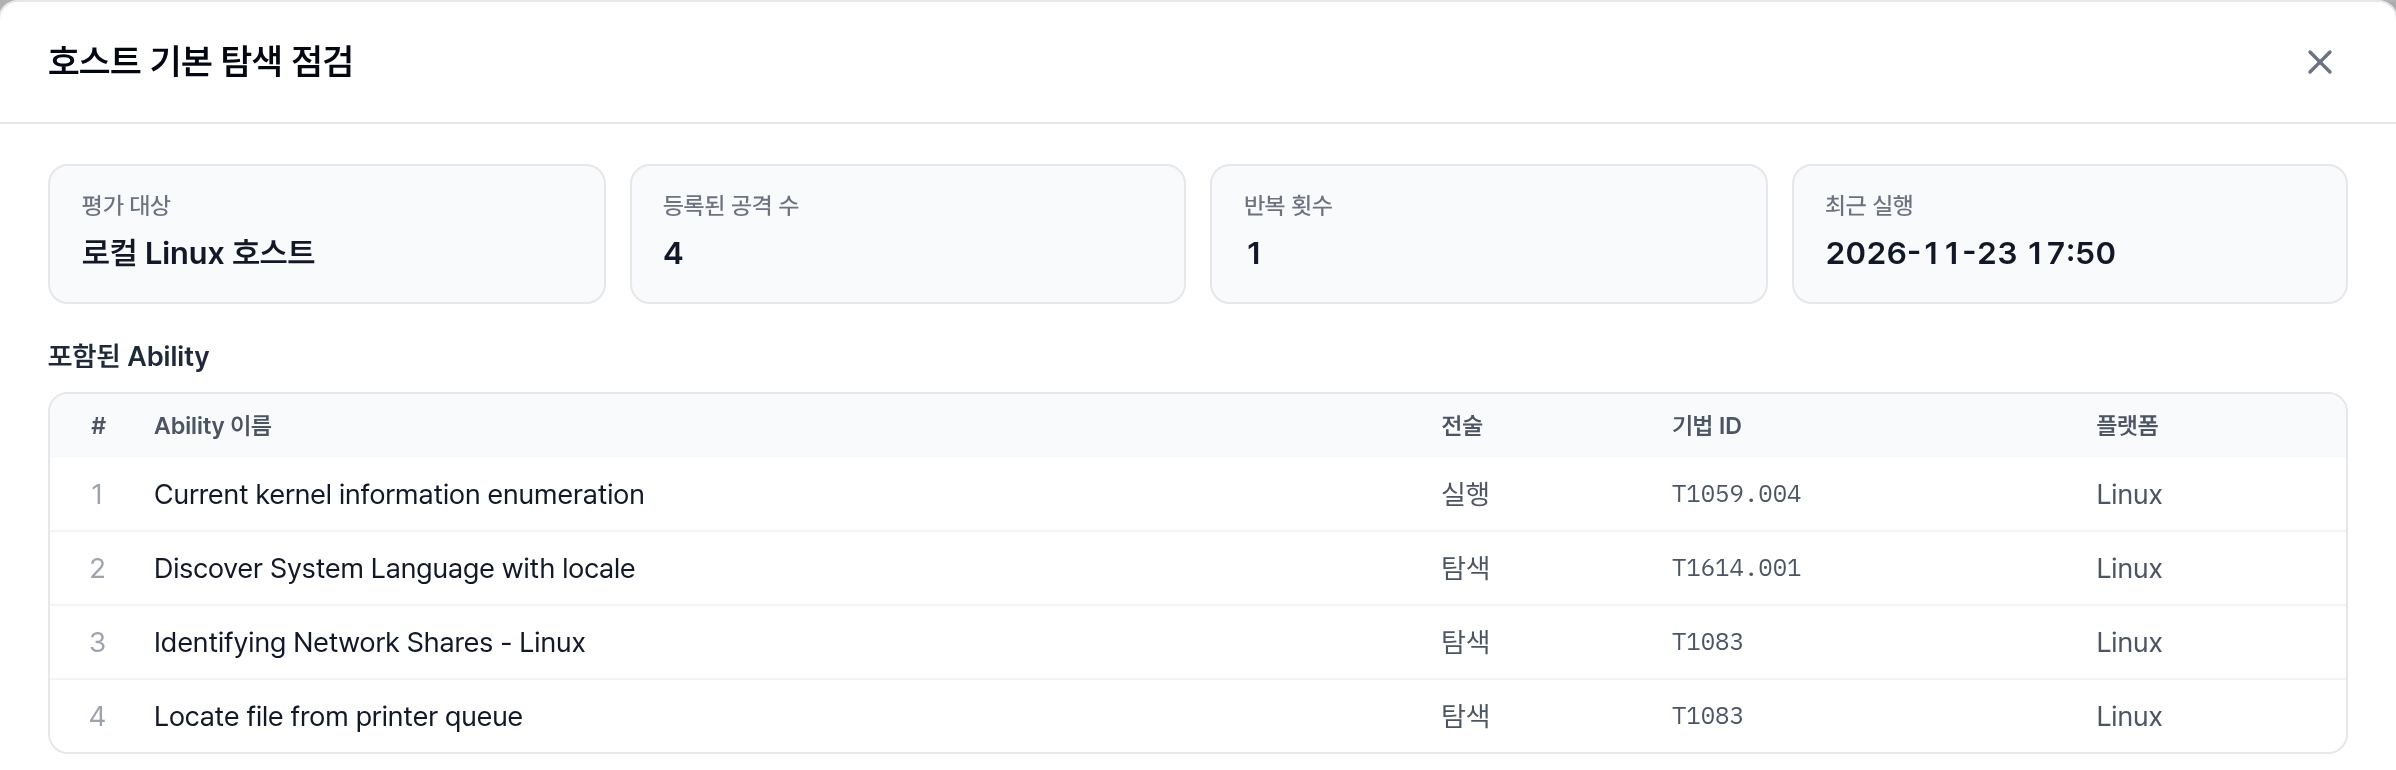
\includegraphics[width=0.62\textwidth]{screenshots-bas/assessment.png}
\caption{평가 상세 화면}
\label{fig:assessment}
\end{figure}

`공격 실행 시작' 버튼을 클릭하면 평가에 등록된 Ability 순서와 대상 에이전트 정보가 미리 입력된 공격 실행 구성 창이 열린다.
운영자는 필요한 추출 규칙과 변수 값을 추가한 뒤 공격 실행을 시작하며, 이때 평가의 `최근 실행' 시각이 기록된다.
평가 기능은 시험 계획을 정의하고 관리하며, 공격 실행 기능은 정의된 계획에 따른 시험 수행 및 결과 기록을 담당한다.
